\section{External Communication}
\label{design:communication}

In \autoref{design:modeler_integration} we established that a bootware adapter in the modeler has to call the local bootware.
From \autoref{design:division} we also know that both the local bootware and the provisioning manager have to call the remote bootware.
We now have to decide, how this external communication with the bootware will work.
There are several factors that impact this decision.
Communication between the components should be as simple as possible, but has to support some critical features.
To keep it simple, it would make sense to use the same communication mechanism for communication between the bootware components as well as with other external components, like the provisioning manager and the bootware adapter.

Since the provisioning processes kicked off by the bootware can potentially take a long time to finish (in the range of minutes to hours), we face possible timeouts when using synchronous communication.
As alternative we could use asynchronous communication with callbacks.
This would avoid timeouts but also creates a new problem.
The callback message send as response is separated from the original message and therefore appears as unsolicited message to the client.
If the client is rejects unsolicited messages, for example because he is located behind a firewall, the callback message might also be blocked.
This could be a problem, since in the environment where the bootware will most likely be used, i.e. at universities, secure networks are very common and asynchronous callbacks could therefore be problematic.
Another solution is to use polling, i.e. after a request was send to the bootware, the bootware is polled periodically for a response.
This also avoids timeouts as well as the firewall problematic.
Disadvantages of polling, for example when many clients poll a server at the same time and cause a bottleneck, will most likely not be a problem in our case, since we only have a very restricted number of clients for each bootware instance and no multi-tenancy.
Since the provisioning process can take very long, there should also be some mechanism to get feedback on the current status during a long running provisioning process.

The communication with the bootware components will contain sensitive data, for example login information for cloud providers.
This information has to be provided from the outside and should be transported securely to prevent malicious or fraudulent attacks.
The selected communication method therefore has to support some sort of security mechanism, ideally end-to-end encryption.
While these security mechanisms will not be used in this thesis due to time constraints, selecting the right communication method is still critical for future development.

Java provides a package for \nom{Remote Method Invocation}{RMI}\footnote{\url{http://docs.oracle.com/javase/7/docs/api/java/rmi/package-summary.html\#package_description}}, which allows objects in one Java VM to invoke methods on objects in another Java VM.
Depending on the implementation, it can be used with polling or asynchronous callbacks.
But since RMI is limited to Java and we might want to communicate with the bootware from a component written in another programming language, RMI doesn't seem like a good fit.
For communication between programs written in different languages we could use the \nom{Common Object Request Broker Architecture}{CORBA}, a standard defined by the \nom{Object Management Group}{OMG}.
It supports mappings for common programming languages, like Java, C++, Python, and others.
CORBA also supports polling and asynchronous method invocation via callbacks~\autocite{corba:async}, as well as transport layer encryption and other security features~\autocite{corba:security}.

As a second alternative, we could communicate with messages by using message-oriented middleware.
As explained earlier in \autoref{fundamentals:service}, it supports communication between different components using adapters and channels.
Asynchronous communication is supported by using message queues for temporary storage.
The middleware can also provide additional persistent storage and backups for high availability~\autocite{mom}.
It may also support security features like encryption.
Another alternative are web services via \nom{Simple Object Access Protocol}{SOAP} or \nom{Representational State Transfer}{REST}.
Like CORBA, web services also support polling and asynchronous invocation, as well as security mechanisms~\autocite{ws:security}.

\begin{figure}[!htbp]
	\centering
	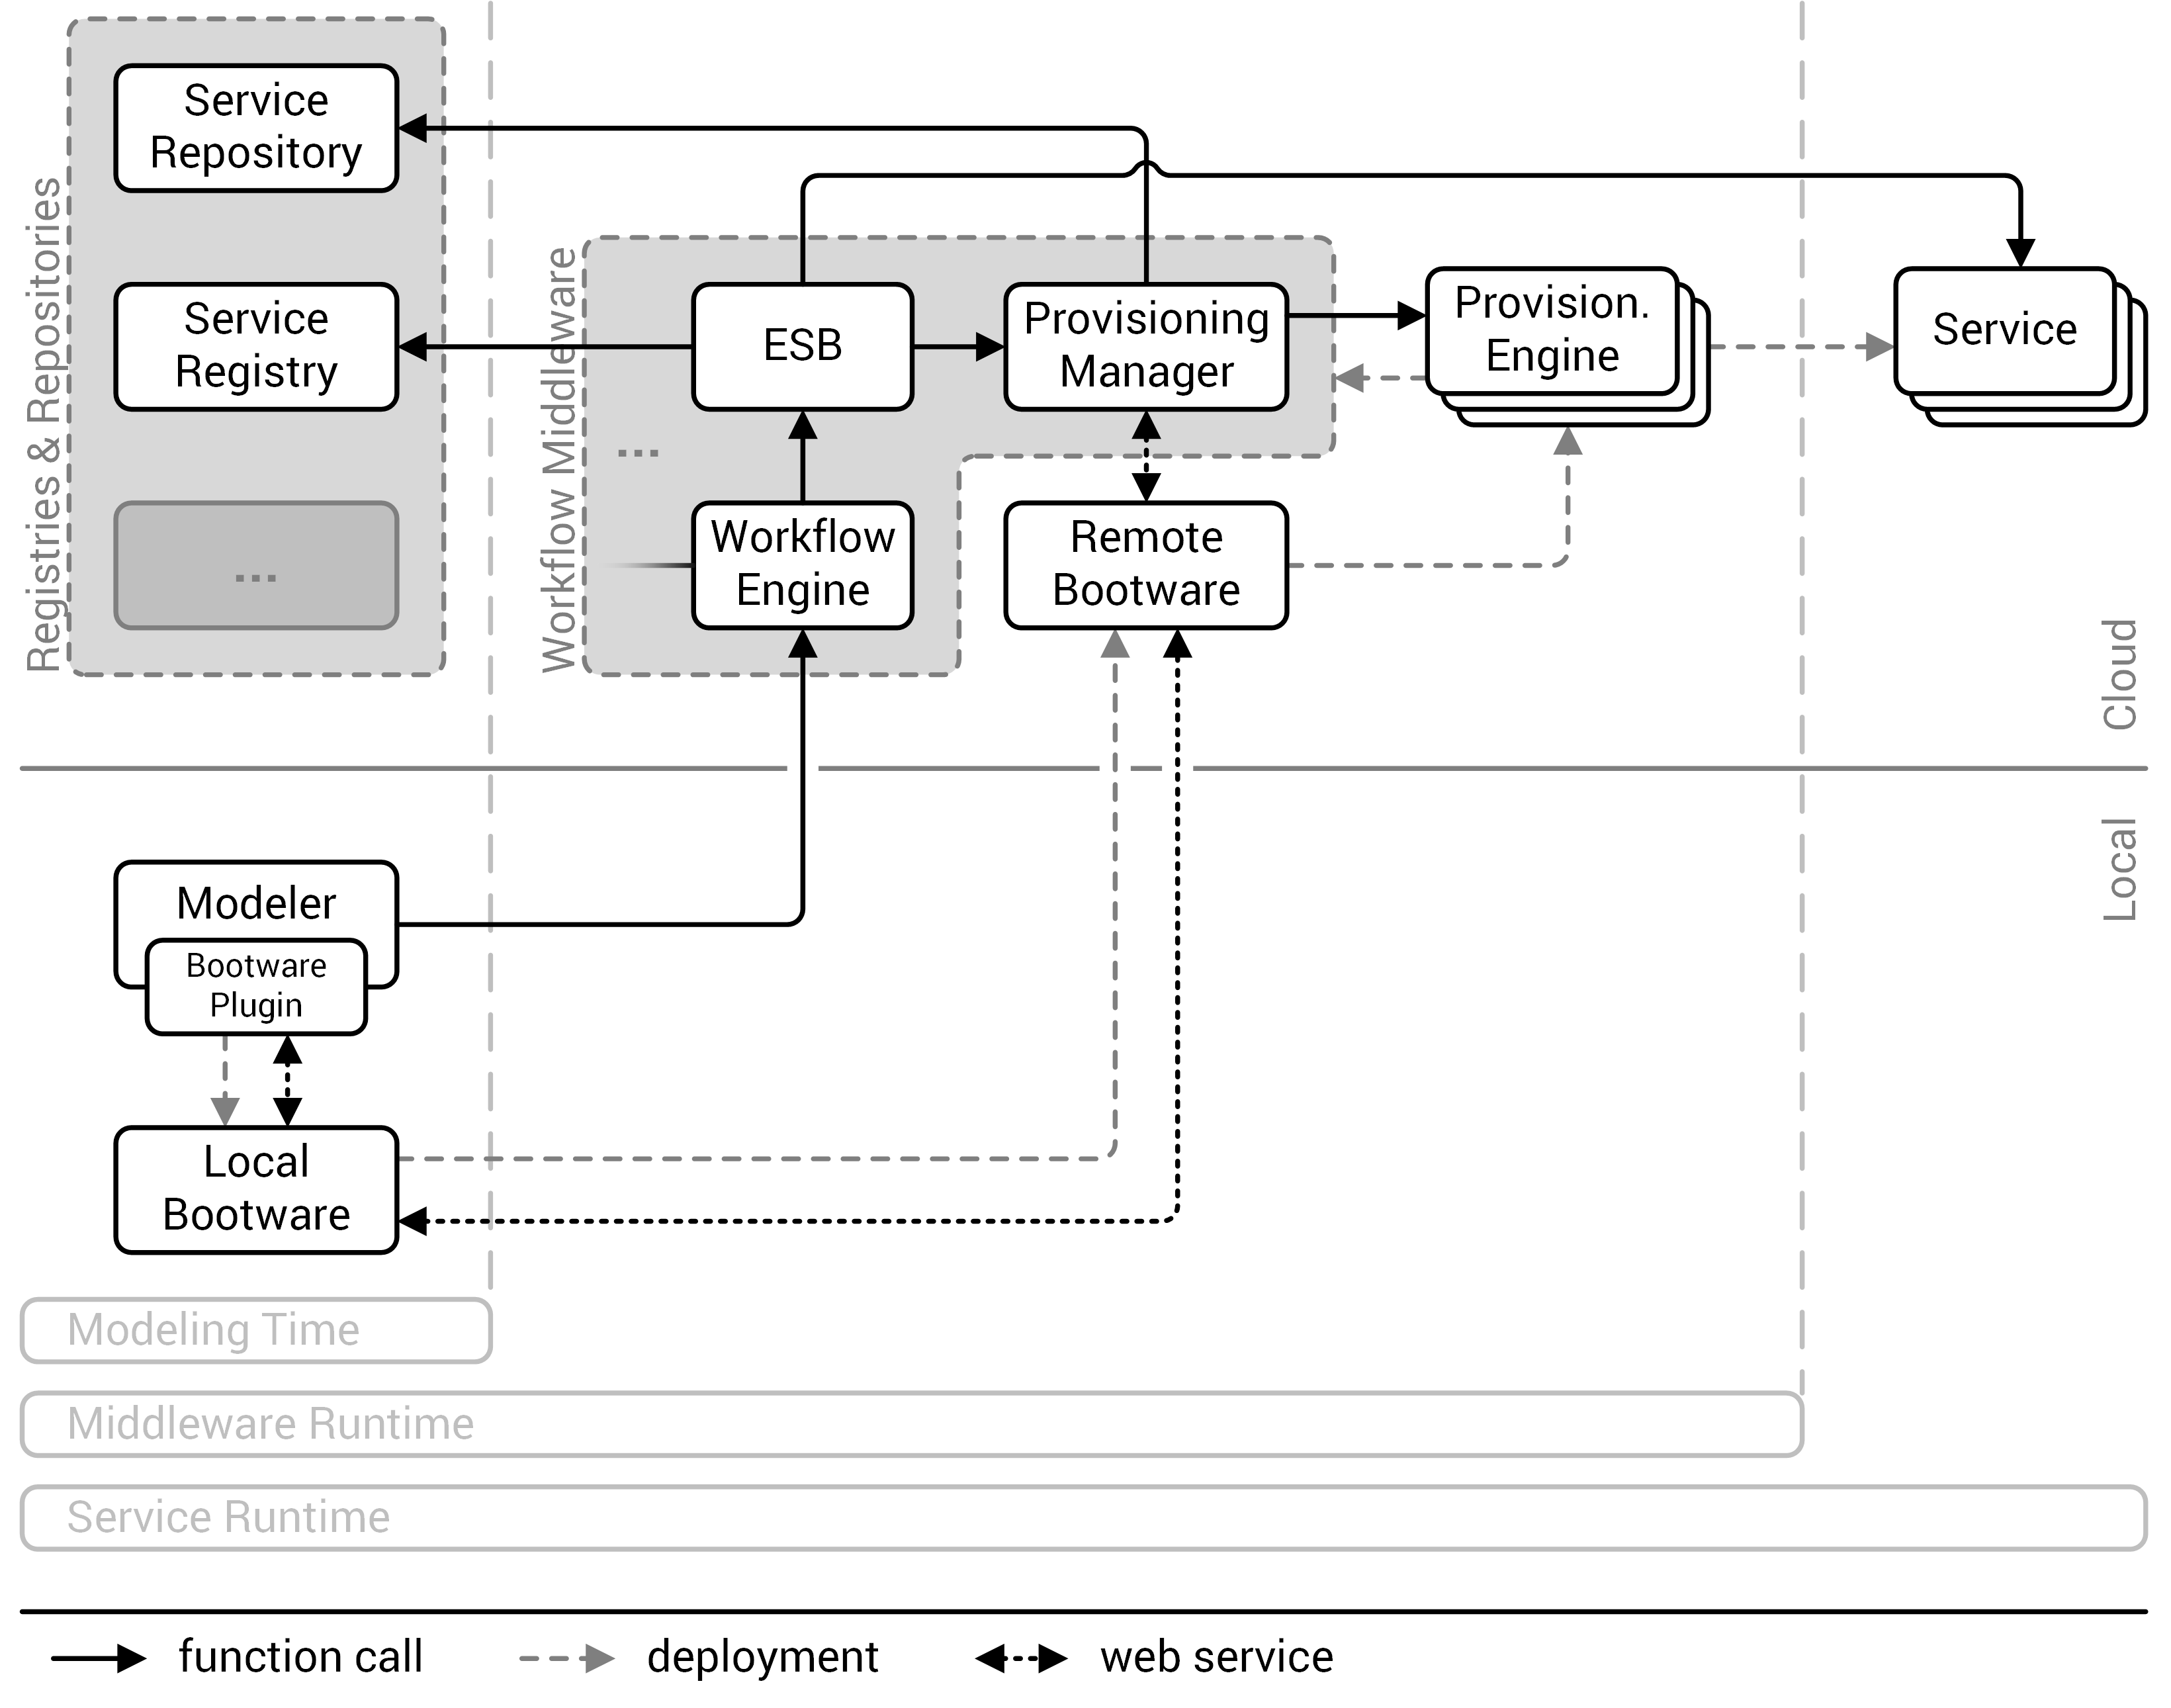
\includegraphics[resolution=600]{design/assets/webservice}
	\caption{Simplified overview of the 2-tier architecture with web service communication}
	\label{image:webservice}
\end{figure}

Since the whole SimTech SWfMS already uses SOAP based web services, it would make sense to also use SOAP based web services as external communication mechanism for the bootware.
The technology and knowledge is already in place and introducing a second mechanism like CORBA would unnecessarily increase the complexity of the project, especially since CORBA doesn't offer any significant advantages over SOAP based web services.
Using a message-oriented middleware would also be an option but introducing another component seems to complicated, especially since we don't need most of the features that it offers (e.g. transactions, persistence, etc.).
\autoref{image:webservice} shows the addition of web service call and return communication between the bootware adapter and the local bootware, and between the remote bootware and the local bootware, as well as the provisioning manager.
With polling, long running provisioning processes won't pose a problem.
We do however still need information during those long running processes to give the user some feedback.
For this, a secondary communication mechanism which supports sending multiple feedback messages has to be used.

\begin{figure}[!htbp]
	\centering
	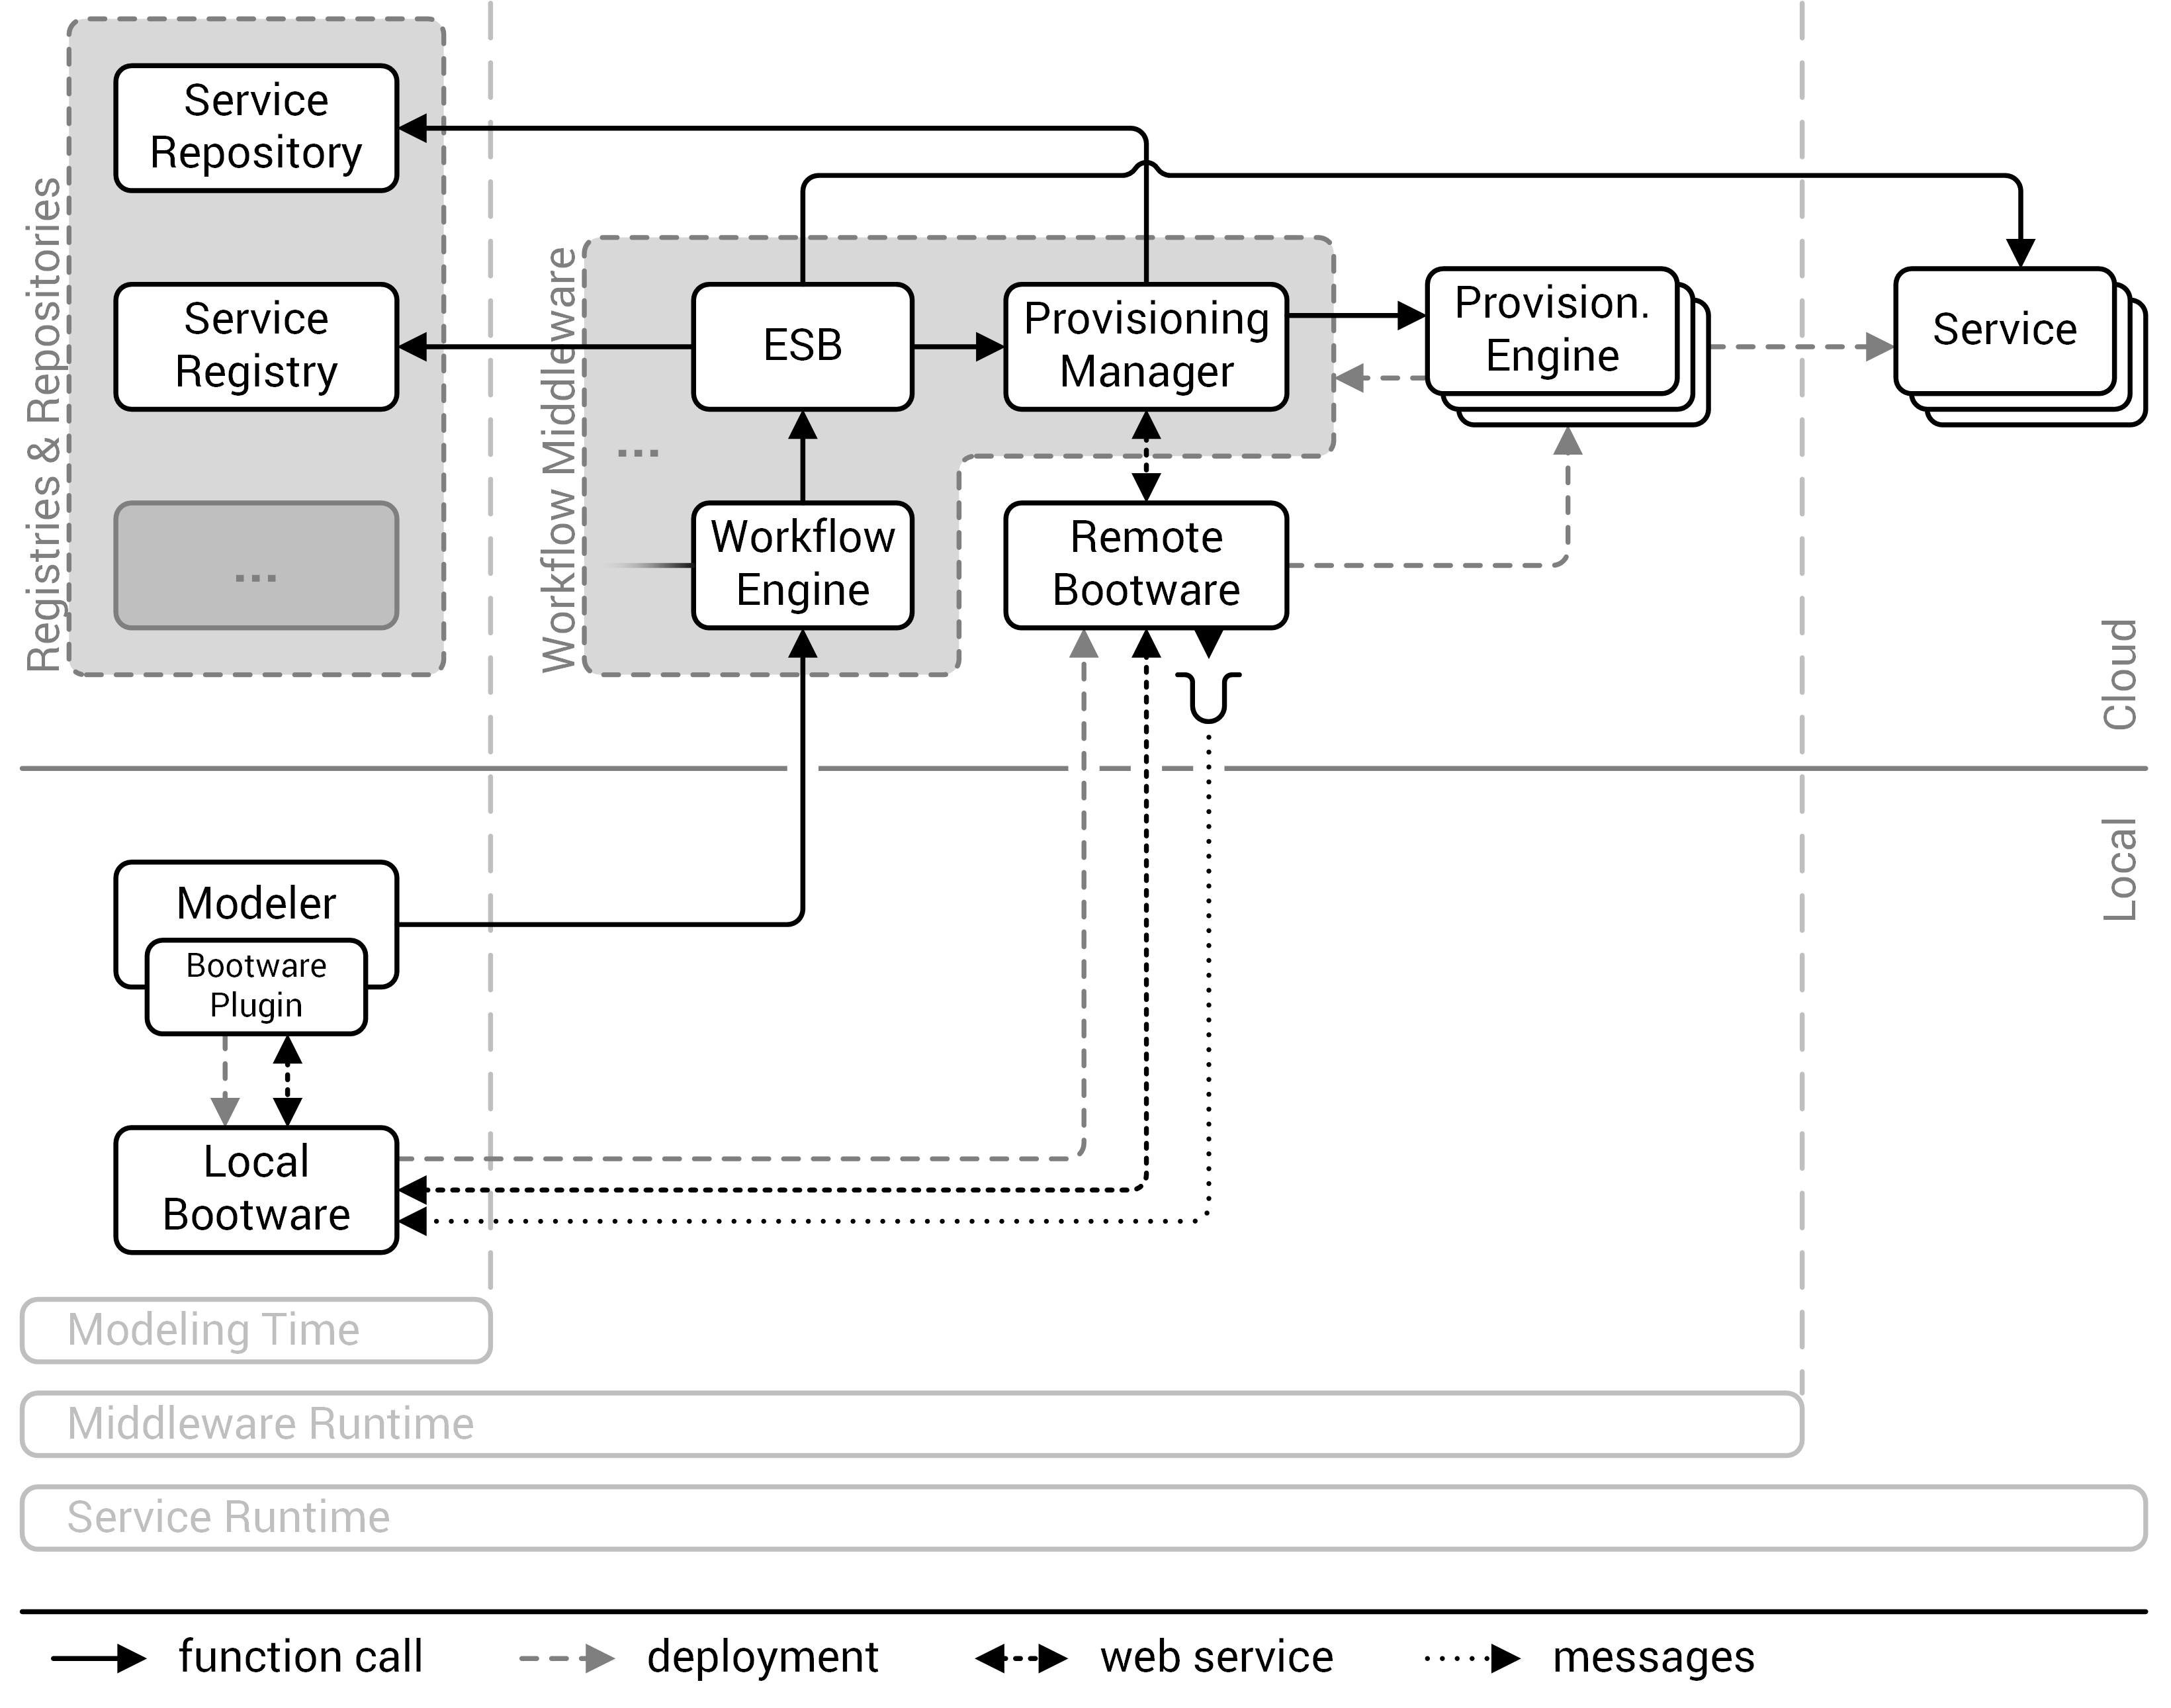
\includegraphics[resolution=600]{design/assets/message_queue}
	\caption{Simplified overview of the 2-tier architecture with web service and messaging queue communication}
	\label{image:message_queue}
\end{figure}

This secondary communication channel could take any form, but a natural choice for publishing the intermediary state of the bootware would be a message queue system.
In this case, the remote bootware pushes messages to a message queue to which the local bootware (and other components if needs be) can subscribe to receive future messages.
\autoref{image:message_queue} shows the proposed architecture with an additional (and optional) message queue that allows the local bootware or other components to listen to status updates from the remote bootware.
Since it is not necessary for the successful use of the bootware, it would make sense to implement this secondary communication mechanism as an extension to the bootware.
This extension would not be part of the core bootware, but rather an additional component that could be used when needed.
This would allow us to add arbitrary communication extensions to the bootware depending on future needs.
How this can be done will be discussed in the next section.
